\documentclass[12pt]{article}

%Paquetes
\usepackage{titlesec}
\usepackage{xcolor}
\usepackage{lipsum}
\usepackage{fontspec}
\usepackage{graphicx} %Imágenes
\usepackage{colortbl}
\usepackage{setspace}
\usepackage[a4paper]{geometry}
\usepackage{fancyhdr}
\usepackage[babel]{csquotes}
\usepackage[spanish, english]{babel}
\usepackage{apacite} % Norma APA bibliografía
\usepackage{natbib} %Bibliografía
\usepackage[nottoc]{tocbibind}
\usepackage[acronym,nonumberlist,toc]{glossaries} %Configuraciones glosario
\usepackage{glossary-superragged} %Configuraciones glosario
\usepackage[hang,flushmargin]{footmisc}
\usepackage{etoolbox}
\usepackage[hidelinks, breaklinks=true]{hyperref}

\usepackage{listings}
\usepackage{color}

\definecolor{dkgreen}{rgb}{0,0.6,0}
\definecolor{gray}{rgb}{0.5,0.5,0.5}
\definecolor{mauve}{rgb}{0.58,0,0.82}

\lstset{frame=tb,
	language=Python,
	aboveskip=3mm,
	belowskip=3mm,
	showstringspaces=false,
	columns=flexible,
	basicstyle={\small\ttfamily},
	numbers=none,
	numberstyle=\tiny\color{gray},
	keywordstyle=\color{blue},
	commentstyle=\color{dkgreen},
	stringstyle=\color{mauve},
	breaklines=true,
	breakatwhitespace=true,
	tabsize=3
}



%Variables
\definecolor{gray80}{gray}{.80}
\definecolor{blueUnir}{HTML}{0098CD}

\geometry{top=2.5cm, bottom=2.5cm, left=3.0cm, right=2.0cm}
\setmainfont{Calibri}
\spacing{1.5} %Interlineado fijo
\setlength{\parskip}{6pt} %6 puntos de espaciado entre párrafos
\setlength{\parindent}{0cm} %Eliminar sangría
\setlength{\footnotesep}{0pt} %Espaciado entre notas
\setlength{\skip\footins}{1.5cm} %Espaciado entre raya y texto
\renewcommand{\footnotelayout}{\small\baselineskip=10pt} % Interlineado sencillo

\fancyhf{}
\pagestyle{fancy}
\rhead[\fontsize{10pt}{12pt}\setmainfont{Calibri Light}\selectfont Nombre del alumno\\Título del trabajo]{\fontsize{10pt}{12pt}\setmainfont{Calibri Light}\selectfont Nombre del alumno\\Título del trabajo} 
\renewcommand{\headrulewidth}{0pt}
%\renewcommand{\footrulewidth}{1pt}
\rfoot[]{\thepage}
\setcounter{tocdepth}{3} 
\setcounter{secnumdepth}{5}
\newcommand\fh{\babelhyphen{hard}}



\titleformat*{\section}{\fontsize{18pt}{18}\selectfont\color{blueUnir}\setmainfont{Calibri Light}} 
\titleformat*{\subsection}{\fontsize{14pt}{14}\selectfont\color{blueUnir}\setmainfont{Calibri Light}} 
\titleformat*{\subsubsection}{\fontsize{12pt}{12}\selectfont\setmainfont{Calibri}\bfseries}

% La forma de definir un acrónimo es la siguiente:
% \newacronym{id}{siglas}{descripción}
% Donde:
% 	'id' es como vas a llamarlo desde el documento.
%	'siglas' son las siglas del acrónimo.
%	'descripción' es el texto que representan las siglas.
%
% Para usarlo en el documento tienes 4 formas:
% \gls{id} - Añade el acrónimo en su forma larga y con las siglas si es la primera vez que se utiliza, el resto de veces solo añade las siglas. (No utilices este en títulos de capítulos o secciones).
% \glsentryshort{id} - Añade solo las siglas de la id
% \glsentrylong{id} - Añade solo la descripción de la id
% \glsentryfull{id} - Añade tanto  la descripción como las siglas


\newacronym{sdr}{SDR}{Software Defined Radio}
%\newacronym{}{}{}
\makeglossaries

\makeatletter
\patchcmd{\@footnotetext}{\footnotesize}{\fontsize{10pt}{12pt}\setmainfont{Calibri}}{}{}
\makeatother

\addto\captionsspanish{%
	\renewcommand*\contentsname{Índice de contenidos}
	\renewcommand{\listtablename}{Índice de tablas} 
	\renewcommand{\tablename}{Tabla} 
	%\renewcommand{\bibname}{Referencia bibliográfica}
}

\titlespacing*{\paragraph}{0pt}{9pt}{0.5ex}
\titleformat{\paragraph}[block]{\normalsize}{\theparagraph}{.5em}{\mdseries}
\titlespacing*{\subparagraph}{0pt}{9pt}{0.5ex}
\titleformat{\subparagraph}[block]{\normalsize}{\thesubparagraph}{.5em}{\mdseries}

\renewenvironment{description}
{\list{}{\labelwidth0pt\itemindent-\leftmargin\parsep0pt\itemsep0pt\let\makelabel\descriptionlabel}}{\endlist}

\begin{document}
	
	\begin{titlepage}
	
	% Quitar dependiendo si título es igual que los demás
	%\newgeometry{top=2.5cm, bottom=2.5cm, left=2.0cm, right=2.0cm}
	
	\centering
	\vspace{3cm}
	
\includegraphics[width=0.60\textwidth]{includes/logoUnir.eps}\\	
	{\Huge Universidad Internacional de La Rioja \\}
	{\LARGE Escuela Superior de Ingeniería y Tecnología \\}
	\vspace{3cm}
	\setmainfont{Calibri Light}
	{\Large máster cursado\\}
	\setmainfont{Calibri}
	{\Huge\textcolor{blueUnir}{título del trabajo} \\}
	%{\Huge\textcolor{blueUnir}{Replay Attack: Propuesta  } \\}
	\vfill{}
	\def\arraystretch{1}
	\setmainfont{Calibri Light}
	\begin{tabular}{| p{8cm} | p{7cm} |}
		\arrayrulecolor{gray80}
		\hline
		Trabajo fin de estudio presentado por: & nombre alumno \\
		\hline
		Tipo de trabajo: & tipo de trabajo \\
		\hline
		Director: & nombre del director \\
		\hline
		Fecha: & fecha del trabajo \\
		\hline
	\end{tabular}
\vspace{4cm}
\end{titlepage}
	\setcounter{page}{2}
	
	\vspace*{\fill}
\selectlanguage{spanish}
\begin{abstract}
	\lipsum[1-1]
\end{abstract}
\textbf{Palabras clave:} Keyword1, Keyword2, Keyword3, Keyword4, Keyword5

\vfill

\selectlanguage{english}

\begin{abstract}
	\lipsum[1-1]
\end{abstract}

\selectlanguage{spanish}
\textbf{Keywords:} Keyword1, Keyword2, Keyword3, Keyword4, Keyword5
\vspace*{\fill}
	\clearpage
	
	\spacing{1.3}
	\setlength{\parskip}{0pt}
	\tableofcontents
	\clearpage
	\listoffigures
	\clearpage
	\listoftables
	\clearpage
	
	\spacing{1.5} %Interlineado fijo
	\setlength{\parskip}{6pt} %6 puntos de espaciado entre párrafos
	
	\section{Introducción}
Ejemplo enumeración:
\begin{enumerate}
	\item Item1
	\item Item2
\end{enumerate}
Aquí se referencia a la imagen \ref{prueba} y aquí a la imagen \ref{prueba_invertida}

Ejemplo figura:
\begin{figure}[h]
	\centering
	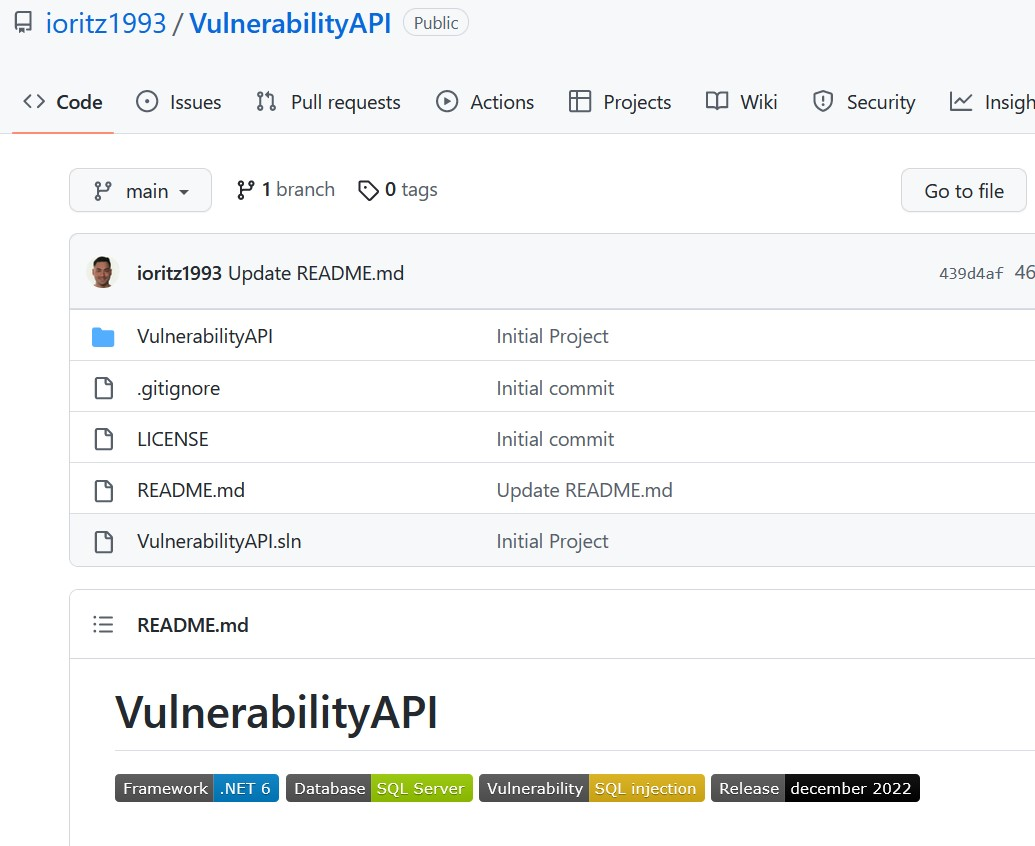
\includegraphics[width=160mm]{includes/ejemplo_figura.jpg}
	\caption[Ejemplo figura]{Ejemplo figura (Elaboración propia)}
	\label{prueba}
\end{figure} 

\begin{figure}[h]
	\centering
	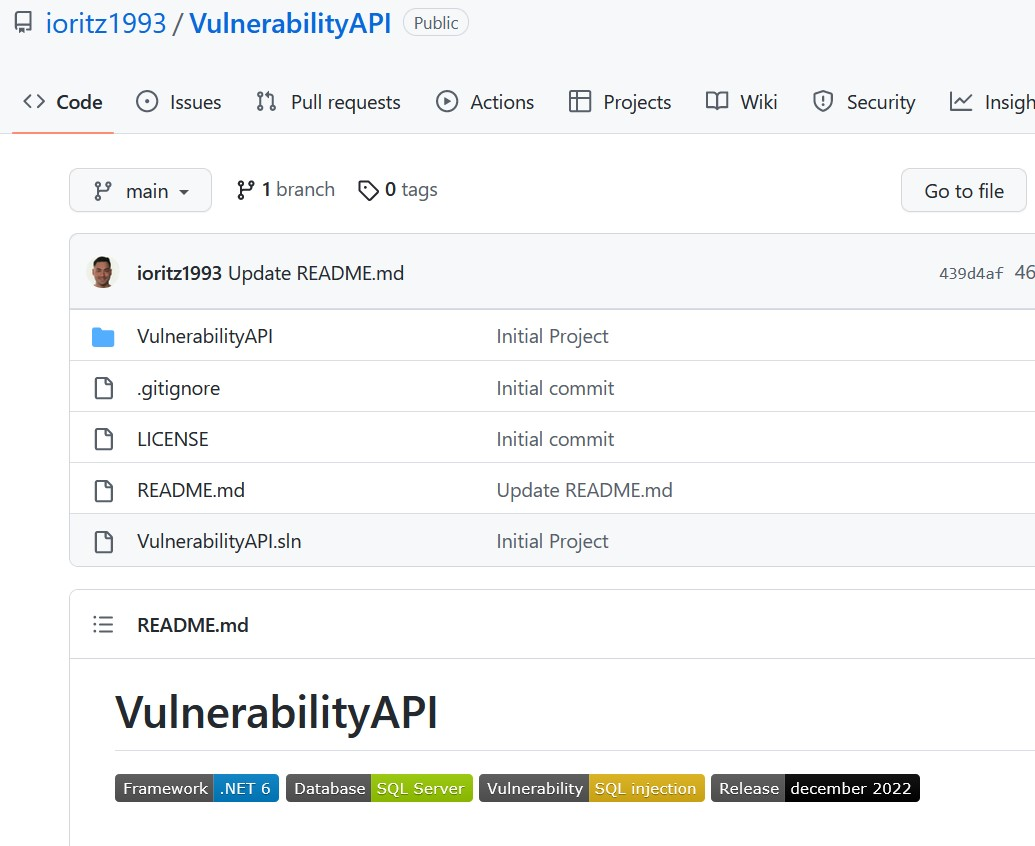
\includegraphics[width=160mm, angle=180]{includes/ejemplo_figura.jpg}
	\caption[Ejemplo figura girada]{Ejemplo figura girada (Elaboración propia)}
	\label{prueba_invertida}
\end{figure} 


	\clearpage
	\section{Justificación}
 Ejemplo referencia \citep{ejemploReferencia}.\par
 Ejemplo acrónimo \gls{sdr}\\
 Ejemplo segunda llamada a acrónimo \gls{sdr}
 Ejemplo tabla \ref{ejemploTabla}
 
 
 \begin{table}[h]
 	\centering
 	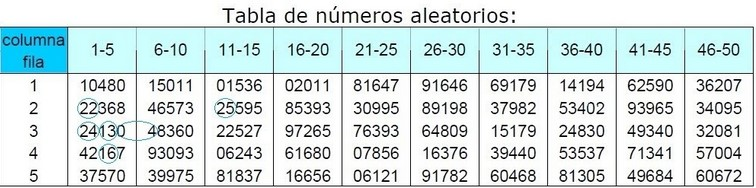
\includegraphics[width=100mm]{includes/ejemplo_tabla.jpg}
 	\caption[Tabla números aleatorios]{Tabla números aleatorios \citep{ejemploReferencia}}
 	\label{ejemploTabla}
 \end{table}
 Como en el caso anterior, la tabla \ref{cochesAfectados} sólo muestra un pequeño porcentaje de coches afectados.
	\clearpage
	\section{Section}
\lipsum[1-1]
\subsection{Subsection}
\lipsum[1-1]

	\clearpage
	\section{Section}
\lipsum[1-1]
\subsection{Subsection}
\lipsum[1-1]
\subsubsection{Subsubsection}
\lipsum[1-1]
\paragraph{Paragraph}
\lipsum[1-1]
\subparagraph{Subparagraph}
\lipsum[1-1]
	\clearpage
	\section{Section}

	\clearpage
	\section{Section}
\lipsum[1-1]

	\clearpage
	\section{Trabajos futuros}
\lipsum[1-1]
	\clearpage
	\section{Conclusiones}
\lipsum[1-1]

	\clearpage
	\printglossary[type=\acronymtype,title={Lista de Acrónimos y Abreviaturas}]
	\glsaddallunused

	\clearpage
	\phantomsection %Insertamos ancla en la bibliografía para hipervínculo
	\begin{flushleft}
		%Visualizar bibliografía con notice incluida la no citada
		\nocite{*}
		\bibliographystyle{apacite}
		\bibliography{recursos/bibliograpfy}
	\end{flushleft}

	\clearpage
	\appendix
	\section{Código de la solución}
\lipsum[1-1]
\subsection{Ejemplo listing}
\begin{lstlisting}
from Functions import Manager

class Key:

	def function(self, parametro):
		if (parametro != 'xxx'):
			raise ValueError("Error");

if __name__ == '__main__':
	rsa = Manager()
	rsa.function()
	print('Prueba listing')
\end{lstlisting}
\end{document} 